% fig-comparator.tex -- float wrapper for fig:comparator.
% Data: thesis_v2/figs/fig-comparator.json, written by thesis_v2/figs/comparator.py from
% RESULTS_cluster/scramble_stratum_audit_v4.json and RESULTS_cluster/re_v3.json.
% Placement: Sections/04a-ruler.tex, immediately after \input of fig-scramble.
% NO width= KEY. The PDF is drawn at 142mm, which is exactly \linewidth in the body block, so
% \includegraphics{} places it at 1.0 and the 10pt type in it prints at 10pt. Adding
% [width=\linewidth] would be harmless today and a silent 11% type shrink the moment the measure
% changes; \resizebox would be wrong at any measure.
\begin{figure}[htbp]
\centering
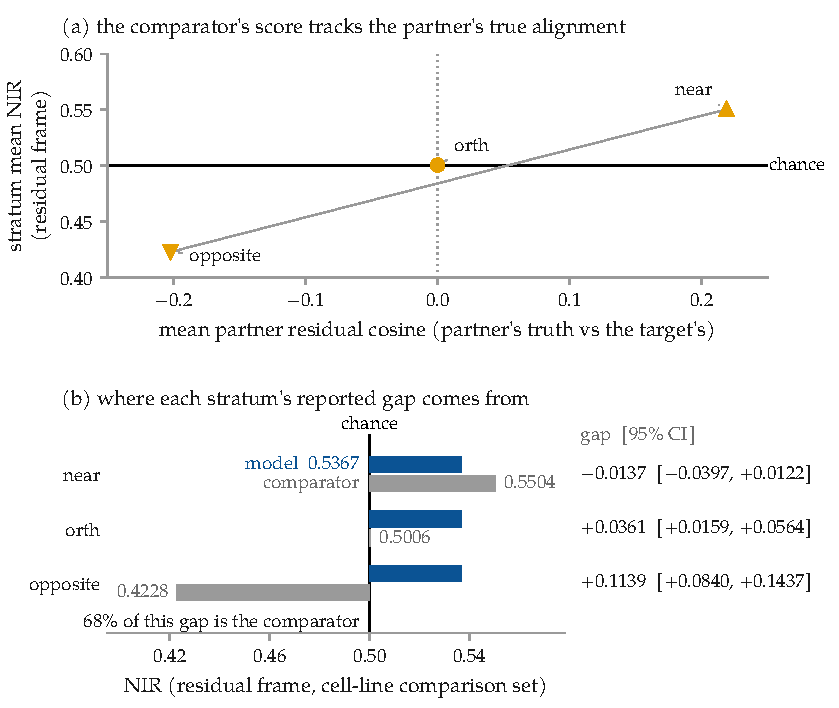
\includegraphics{fig-comparator}
% Short caption: 46 characters, and it states the finding rather than the topic. The long form
% below carries the calibration half of the argument; the List of Figures gets the consequence.
\caption[Most of the \texttt{opposite} gap is the comparator]{%
\textbf{The comparator's own score is a monotone function of how correct the swapped-in partner
is, so most of the \texttt{opposite} stratum's headline gap is the comparator failing rather than
the model knowing.} All quantities are residual-frame $\NIR$ scored against the cell-line
comparison set, pooled over the $\num{1394}$ scored conditions.
\emph{(a)} Each mark is one swap stratum, at its mean partner residual cosine and its mean
$\NIR$. The score falls from $0.5504$ through $0.5006$ to $0.4228$ as the partner's true residual
moves from aligned to anti-aligned, so \texttt{near} hands the model a partly correct answer and
\texttt{opposite} an actively wrong one. The straight line is the chord joining the two extreme
marks, drawn as a guide to the eye; it is not a fit, and \texttt{orth} lies $0.016$ above it.
Because the strata are defined using the \emph{true} residual geometry, \texttt{orth}'s sitting on
chance is an empirical property of this sample and not an independently established null: it is
the least contaminated comparator available, which is a weaker statement
(\cref{sec:res-generalisation}).
\emph{(b)} The same gap $\gap$ split at chance into its two terms,
$\gap = (\NIR_{\textrm{model}} - 0.5) + (0.5 - \NIR_{\textrm{scramble}})$. The accent bar is the
model's own advantage over chance, $+0.0367$, and is identical on all three rows because it is the
same model arm; the strata differ only in the grey bar, the comparator's own displacement from
chance, drawn on the side it actually falls --- right of the rule it subtracts from the gap, left
of the rule it adds. On \texttt{opposite} the grey term is $+0.0772$ of the $+0.1139$ reported,
$68\%$ of it, which is the annotation on that row.
Intervals are $95\%$ two-way cluster-robust on cell line and treatment well ($42$ cell lines,
$200$ wells); the one-way variants stored alongside them are not drawn.}
\label{fig:comparator}
\end{figure}
